\subsection{Введение}
Для эффективного исследования пещер необходимо выставить требования к разрабатываемому роботу. На основании литературного обзора было решено, что робот должен:
\begin{enumerate}
    \item иметь малые габариты, чтобы иметь возможность пролезать через щели в скальной породе и не застревать среди камней;
    \item обладать достаточной проходимостью по сыпучим грунтам;
    \item иметь возможность преодолевать малые водные преграды;
    \item мог взбираться на большие каменные уступы.
\end{enumerate}

Было решено, что цикловой движитель с одной степенью свободы в ноге лучше всего подходит для решения подобных задач.


\subsection{Решение задачи структурного синтеза}
Для цикловых движителей с одной степенью свободы в ноге вопрос о количестве ног не имеет однозначного решения. Поэтому необходимо провести структурный синтез, чтобы определить их количество. Данная задача решалась с помощью генетического алгоритма.

Генетический алгоритм это эвристический алгоритм поиска, используемый для решения задач оптимизации и моделирования путём случайного подбора, комбинирования и вариации искомых параметров с использованием механизмов, аналогичных естественному отбору в природе. Для решения задачи использовалась библиотека Deap.

Геометрическая модель робота представлена в виде трехмерного параллелепипеда с несколькими ногами $\gamma$ с каждой стороны. Каждая нога имеет постоянное смещение угла поворота относительно своей соседней ноги $\alpha$ \pic{fig:best_gen_robot.jpg}.

\begin{figure}[H]
    \centering
    \begin{tikzpicture}
        % Include the image in a node
        \node [above right, inner sep=0] (image) at (0,0)
        {\centering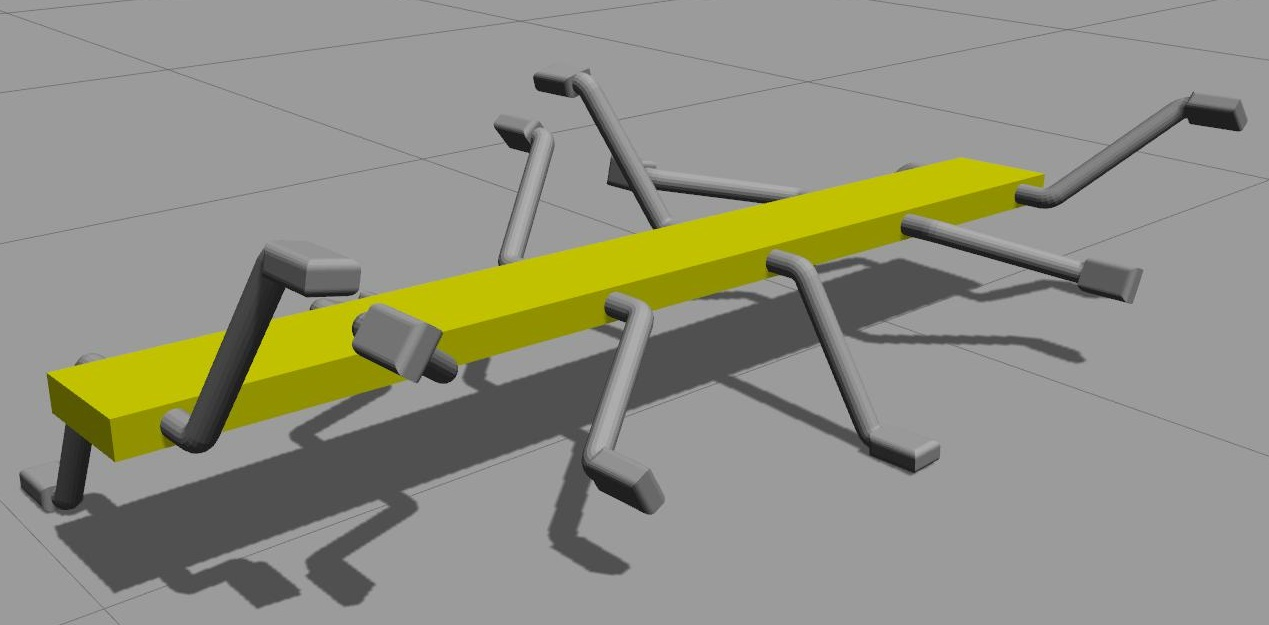
\includegraphics[height=3cm,width=1\textwidth,keepaspectratio]{best_gen_robot.jpg}};
        % Create scope with normalized axes
        \begin{scope}[
                x={($ 0.1*(image.south east)$)},
                y={($ 0.1*(image.north west)$)}]
            % Labels
            \draw [green, very thick,
                decorate,
                decoration = {brace,
                        raise=5pt,
                        amplitude=5pt,
                        aspect=0.5}] (1.4,3.6) --  (8.1,6.8)
            node[rounded corners=3pt, pos=0.5,above left =14pt,black,fill=white]{\tiny $(\gamma - 1) h_{\text{leg}}sin(\alpha)$};

            \draw[stealth-, very thick,green] (9.5,7.8) -- (7.8,1.94);
            \draw[stealth-, very thick,green] (1.5,2.8) -- (7,1)
            node[rounded corners=3pt,right,black,fill=white]{\tiny $\gamma = 6$};

            \draw[thin,green] (6.7,4) -- (5.75,9);
            \draw[thin,green] (4.85,3.5) -- (5.75,9);
            \draw[thin,green,stealth-stealth] (6.32,6) arc (-79.2:-99.2:3) node [rounded corners=3pt,below = 2pt,black,fill=white, midway] {\tiny $\alpha$};
        \end{scope}
    \end{tikzpicture}
    \caption{Объяснение параметров, участвующих в описании индивида в популяции}
    \label{fig:best_gen_robot.jpg}
\end{figure}

Эту задачу можно сформулировать как мультикритериальную задачу оптимизации, где мы пытаемся максимизировать дистанцию, пройденную за фиксированное время, и минимизировать длину робота \eqref{eq:second}. Параметрами индивида являлись $\gamma$ и $\alpha$.

\begin{eqnarray}
    \label{eq:second}
    F \rightarrow max = \beta \left( {\omega}_{1} \cdot \overbrace{\delta}^{\text{Distance}} + {\omega}_{2} \cdot \overbrace{\frac{1}{(\gamma - 1) h_{\text{leg}}sin(\alpha)}}^{\text{Simplified body length}}\right) + \\ \nonumber + (1 - \beta) {\delta}^{{\omega}_{1}} {\left( \frac{1}{(\gamma - 1)h_{\text{leg}}sin(\alpha)}\right)}^{{\omega}_{2}}
\end{eqnarray}
где $\delta$ дистанция, $\beta$ адаптивный параметр, ${\omega}_{1,2} \in  [ 0..1 ] $ весовые коэффициенты.



Весовые коэффициенты настраивались в зависимости от выбора приоритета. Невзирая на выбранные коэффициенты, оптимальным набор лапок начинался с 8-ми и заканчивался 14-ью. Это объясняется критерием статического равновесия, который, как оказалось, увеличивает проходимость механизма. В данном случае 4 лапки всегда будут касаться пола. 

Было проведено два испытания. На первом испытании мы стремились найти только одного лучшего робота, только для местности T1 \pic{fig:terrain_1}. На втором этапе мы хотели видеть зависимость от разных типов ландшафтов при меньшем количестве индивидуальностей.

Первый этап: каждый робот проходил 10 разных ландшафтов по 9 секунд каждую. Вторая фаза: она имеет те же параметры, что и первая фаза, но с измененным размером популяции. 

В соответствии с таблицей \ref{tabular:Table2} (весовые коэффициенты равны 0.6 и 0.4 соответственно) видно, что мы имеем сходимость в параметрах дизайна. \href{https://youtu.be/DcovvkTZgsg}{Видео прохождения препятствия лучшим индивидом}.

\begin{figure}[h]
    \begin{subfigure}{0.33\textwidth}
    \centering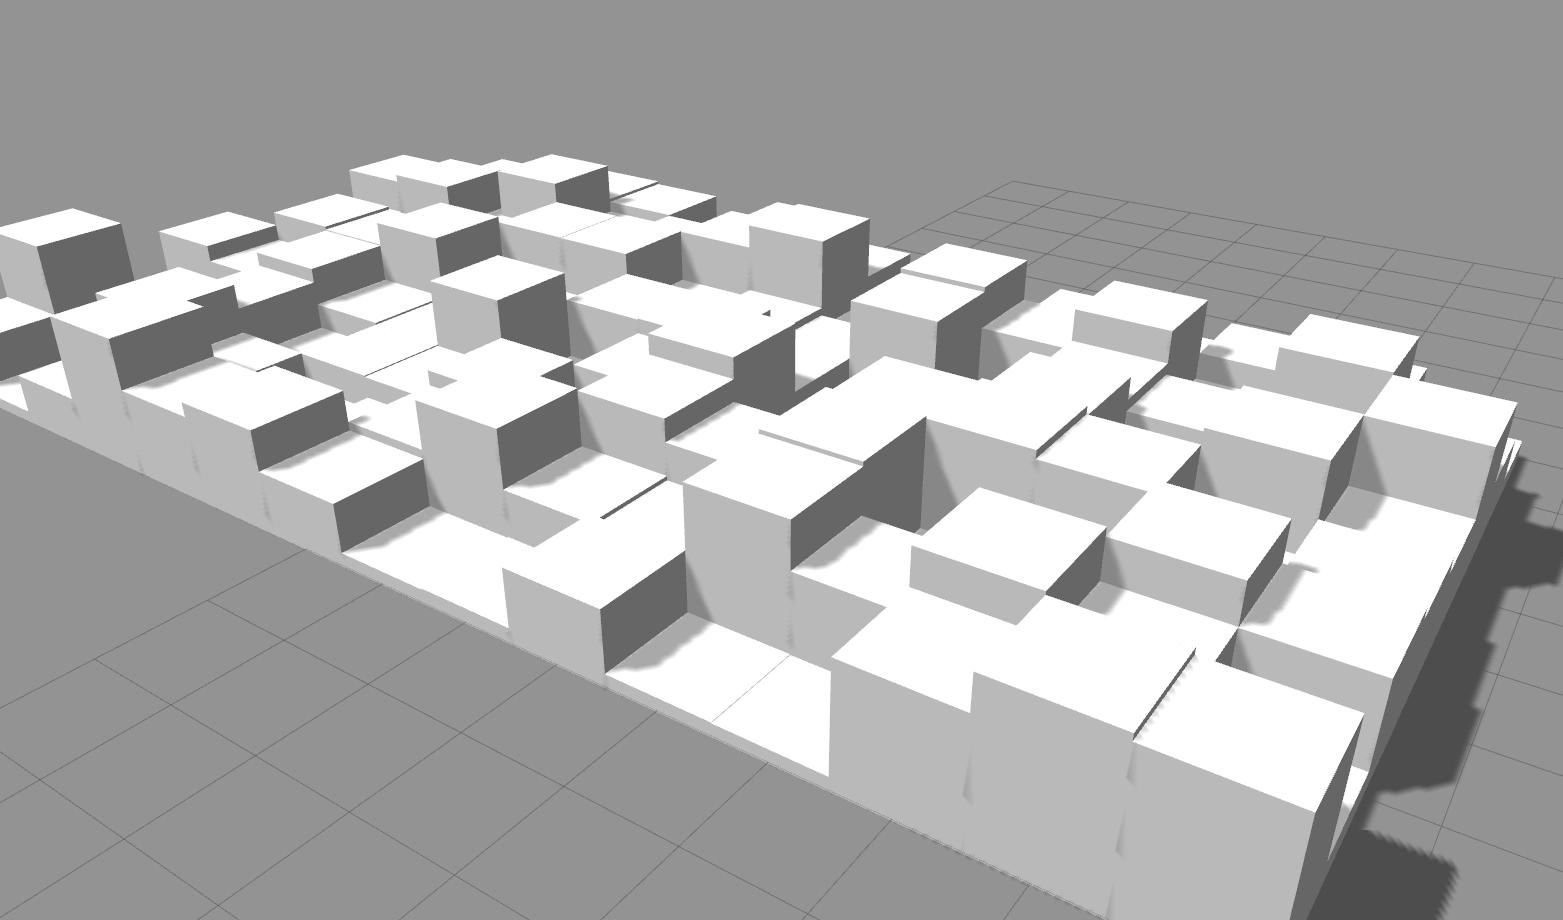
\includegraphics[width=0.8\textwidth]{terrain_1} 
    \caption{T1: 3D-боксы с равномерным распределением высоты}
    \label{fig:terrain_1}
    \end{subfigure}
    \begin{subfigure}{0.33\textwidth}
    \centering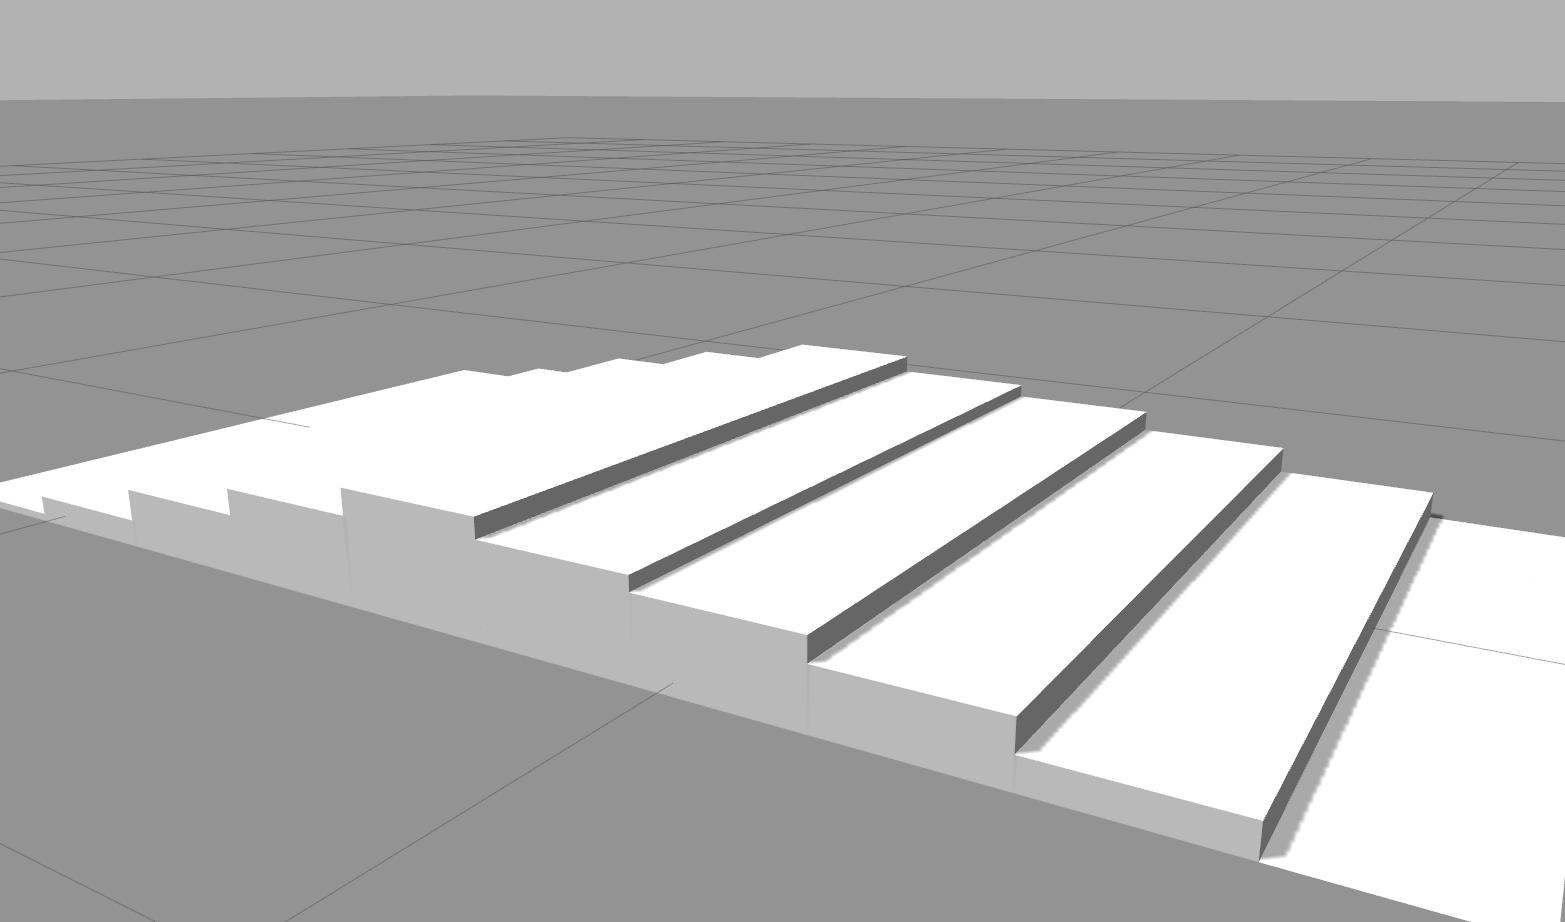
\includegraphics[width=0.8\textwidth]{terrain_2} 
    \caption{T2: 2D-полосы с гауссовой функциональной высотой}
    \label{fig:terrain_2}
    \end{subfigure}
    \begin{subfigure}{0.33\textwidth}
    \centering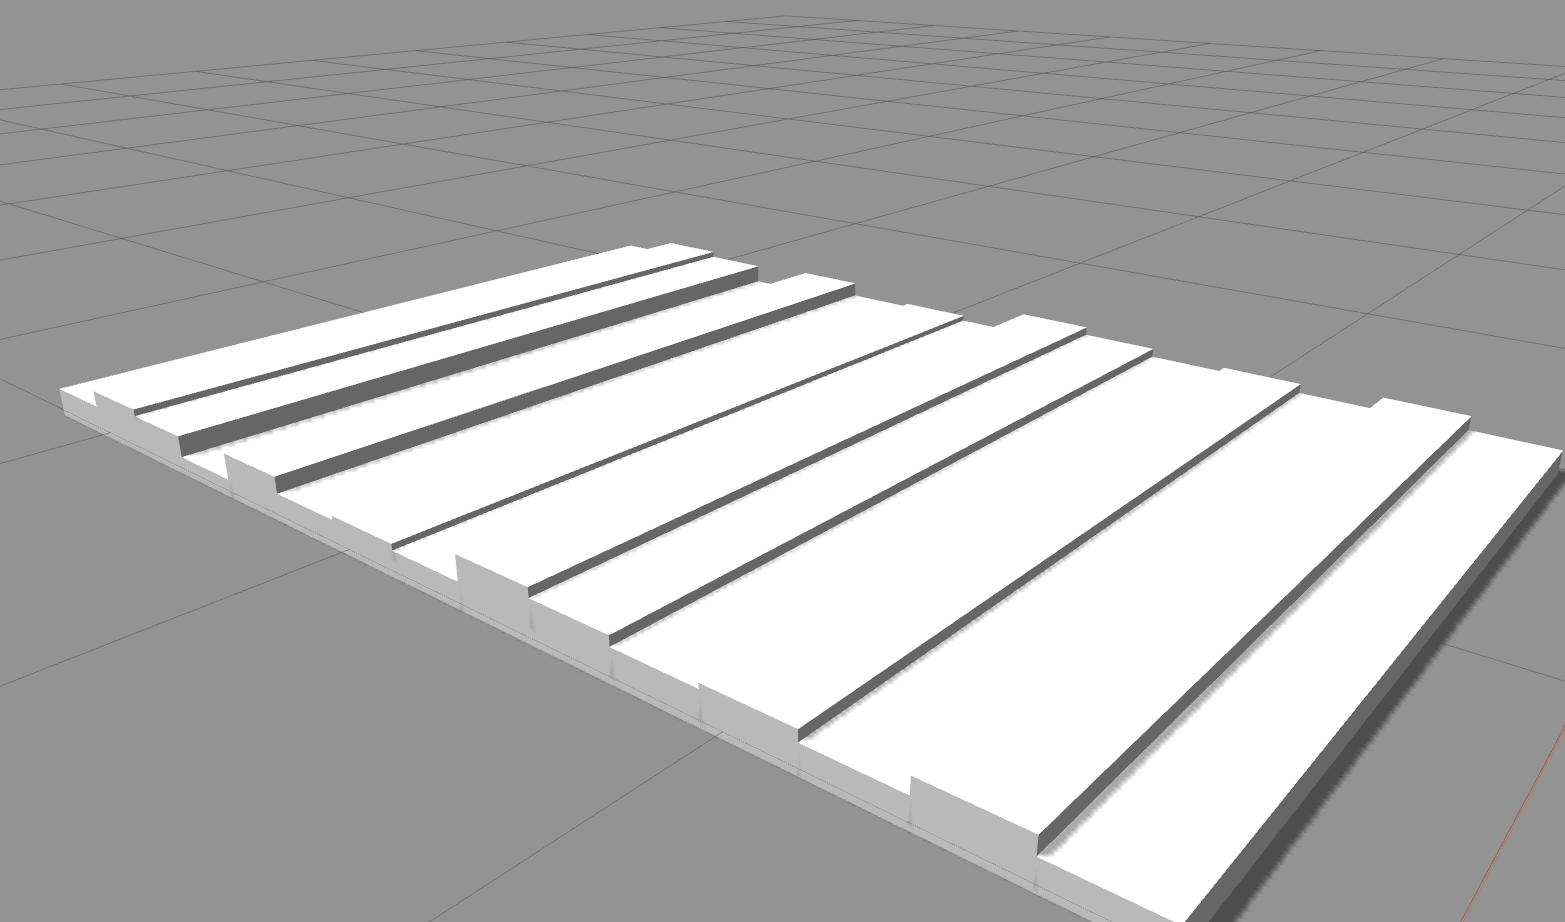
\includegraphics[width=0.8\textwidth]{terrain_3}
    \caption{T3: 2D-полосы с распределением высоты по гауссовской функции)}
    \label{fig:terrain_3}
    \end{subfigure}
     
    \caption{Примеры сгенерированных территорий}
    \label{fig:terrains}
\end{figure}
\vspace{-0.5cm}

\begin{table}[H]
\caption{Зависимость между статистикой значения пригодности (средняя, std) и типами ландшафта}
\label{tabular:Table2}
\begin{center}
\begin{tabular}{c|c|c|c}

\textbf{\makecell{Территория, популяция}} & \textbf{\makecell{Параметры}} & \textbf{\makecell{Среднее \\значение }} & \textbf{\makecell{Std \\целевая функция}}\\
\hline
\textbf{\makecell{T1 \pic{fig:terrain_1}, 110}} & \makecell{(6, 72)} & \makecell{2.38} & \makecell{0.34}
\\
\textbf{\makecell{T2 \pic{fig:terrain_2}, 55}}& \makecell{(5, 68)} & \makecell{1.95} & \makecell{0.35} 
\\
\textbf{\makecell{T3 \pic{fig:terrain_3}, 55}} & \makecell{(6, 77)} &  \makecell{2.08} & \makecell{0.33} \\
\hline
\end{tabular}
\end{center}
\end{table}

\subsection{Концепт движения циклового движителя вбок без смены ориентации}

Одно из требований было, чтобы робот мог проходить сквозь узкие пространства и не застревать при поворотах. Проблема застревания решается с помощью изменения угла между лапкой и корпусом робота.

\begin{figure}[H]
    \centering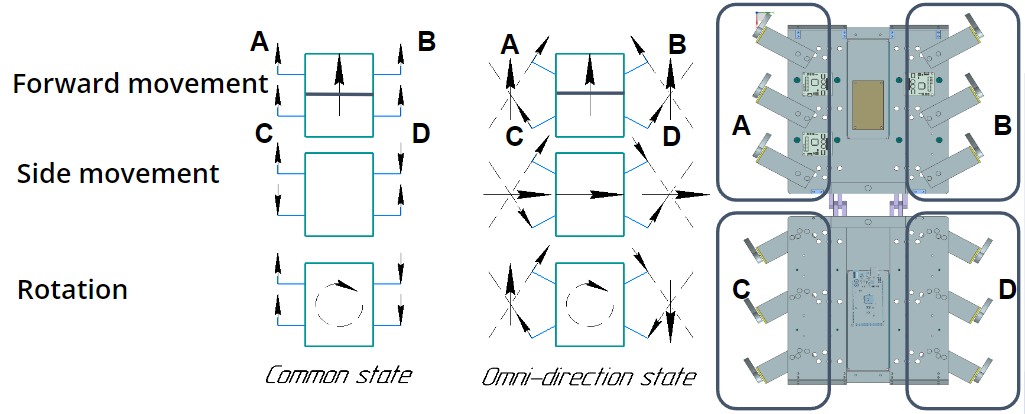
\includegraphics[height=3.5cm,width=1\textwidth,keepaspectratio]{omni_rot.png}
    \caption{Векторное представление сил в классическом и всенаправленном состоянии}
    \label{fig:omnidirection}
\end{figure}

На рисунке \ref{fig:omnidirection} представлена иллюстрация данной концепции: для того, чтобы робот двигался во всех направлениях, необходимо разбить его лапки на группы, чтобы получилось 4 группы. Данные группы на рисунке названы A-D. То есть в каждую группу вошли по 3 лапки, с каждой стороны одного сегмента.

Если сравнивать с классической компоновкой роботов (угол между корпусом робота и осью вала привода лапки равен 90 градусов), то вектор внешних сил будет таким, как на левой части Рис. \ref{fig:omnidirection}. Стрелка в центре робота — суперпозиция всех сил. Если изменить угол оси привода лапок в соответствии с предлагаемой концепцией, то возможно получить значения суперпозиции сил, представленные на Рис. \ref{fig:omnidirection} в центре. То есть, чтобы переместить корпус робота направо, группы А и D должны вращать лапки в одну сторону, а группы C и B — в противоположную. Правая часть рисунка иллюстрирует расположение групп лапок на исследуемом роботе. 

\subsection{Разработка итераций}
Робот разрабатывался итеративно и на основе новых данных создавалась новая концепция. Основные плюсы и недостатки итераций представлены в таблице \ref{tabular:robot_comparison}.

Концептуально было замечено, что высота лапки и наличие сегмента разительно влияет на проходимость конструкции. \href{https://youtu.be/EQ6oGZVDpoc}{Демонстрационное видео}.

\begin{figure}[H]
    \centerfloat{
        \hfill
        \subcaptionbox[List-of-Figures entry]{Первая итерация\label{fig:strirus_0}}{%
            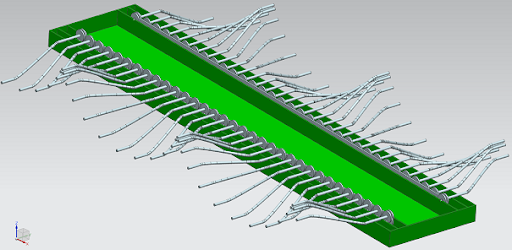
\includegraphics[width=0.33\linewidth]{strirus_0.png}}
        \hfill
        \subcaptionbox[List-of-Figures entry]{Вторая итерация \label{fig:strirus_1}}{%
            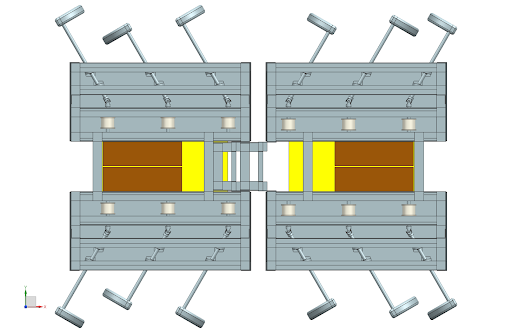
\includegraphics[width=0.33\linewidth]{strirus_1.png}}
        \hfill
        \subcaptionbox{Третья итерация\label{fig:strirus_2}}{%
        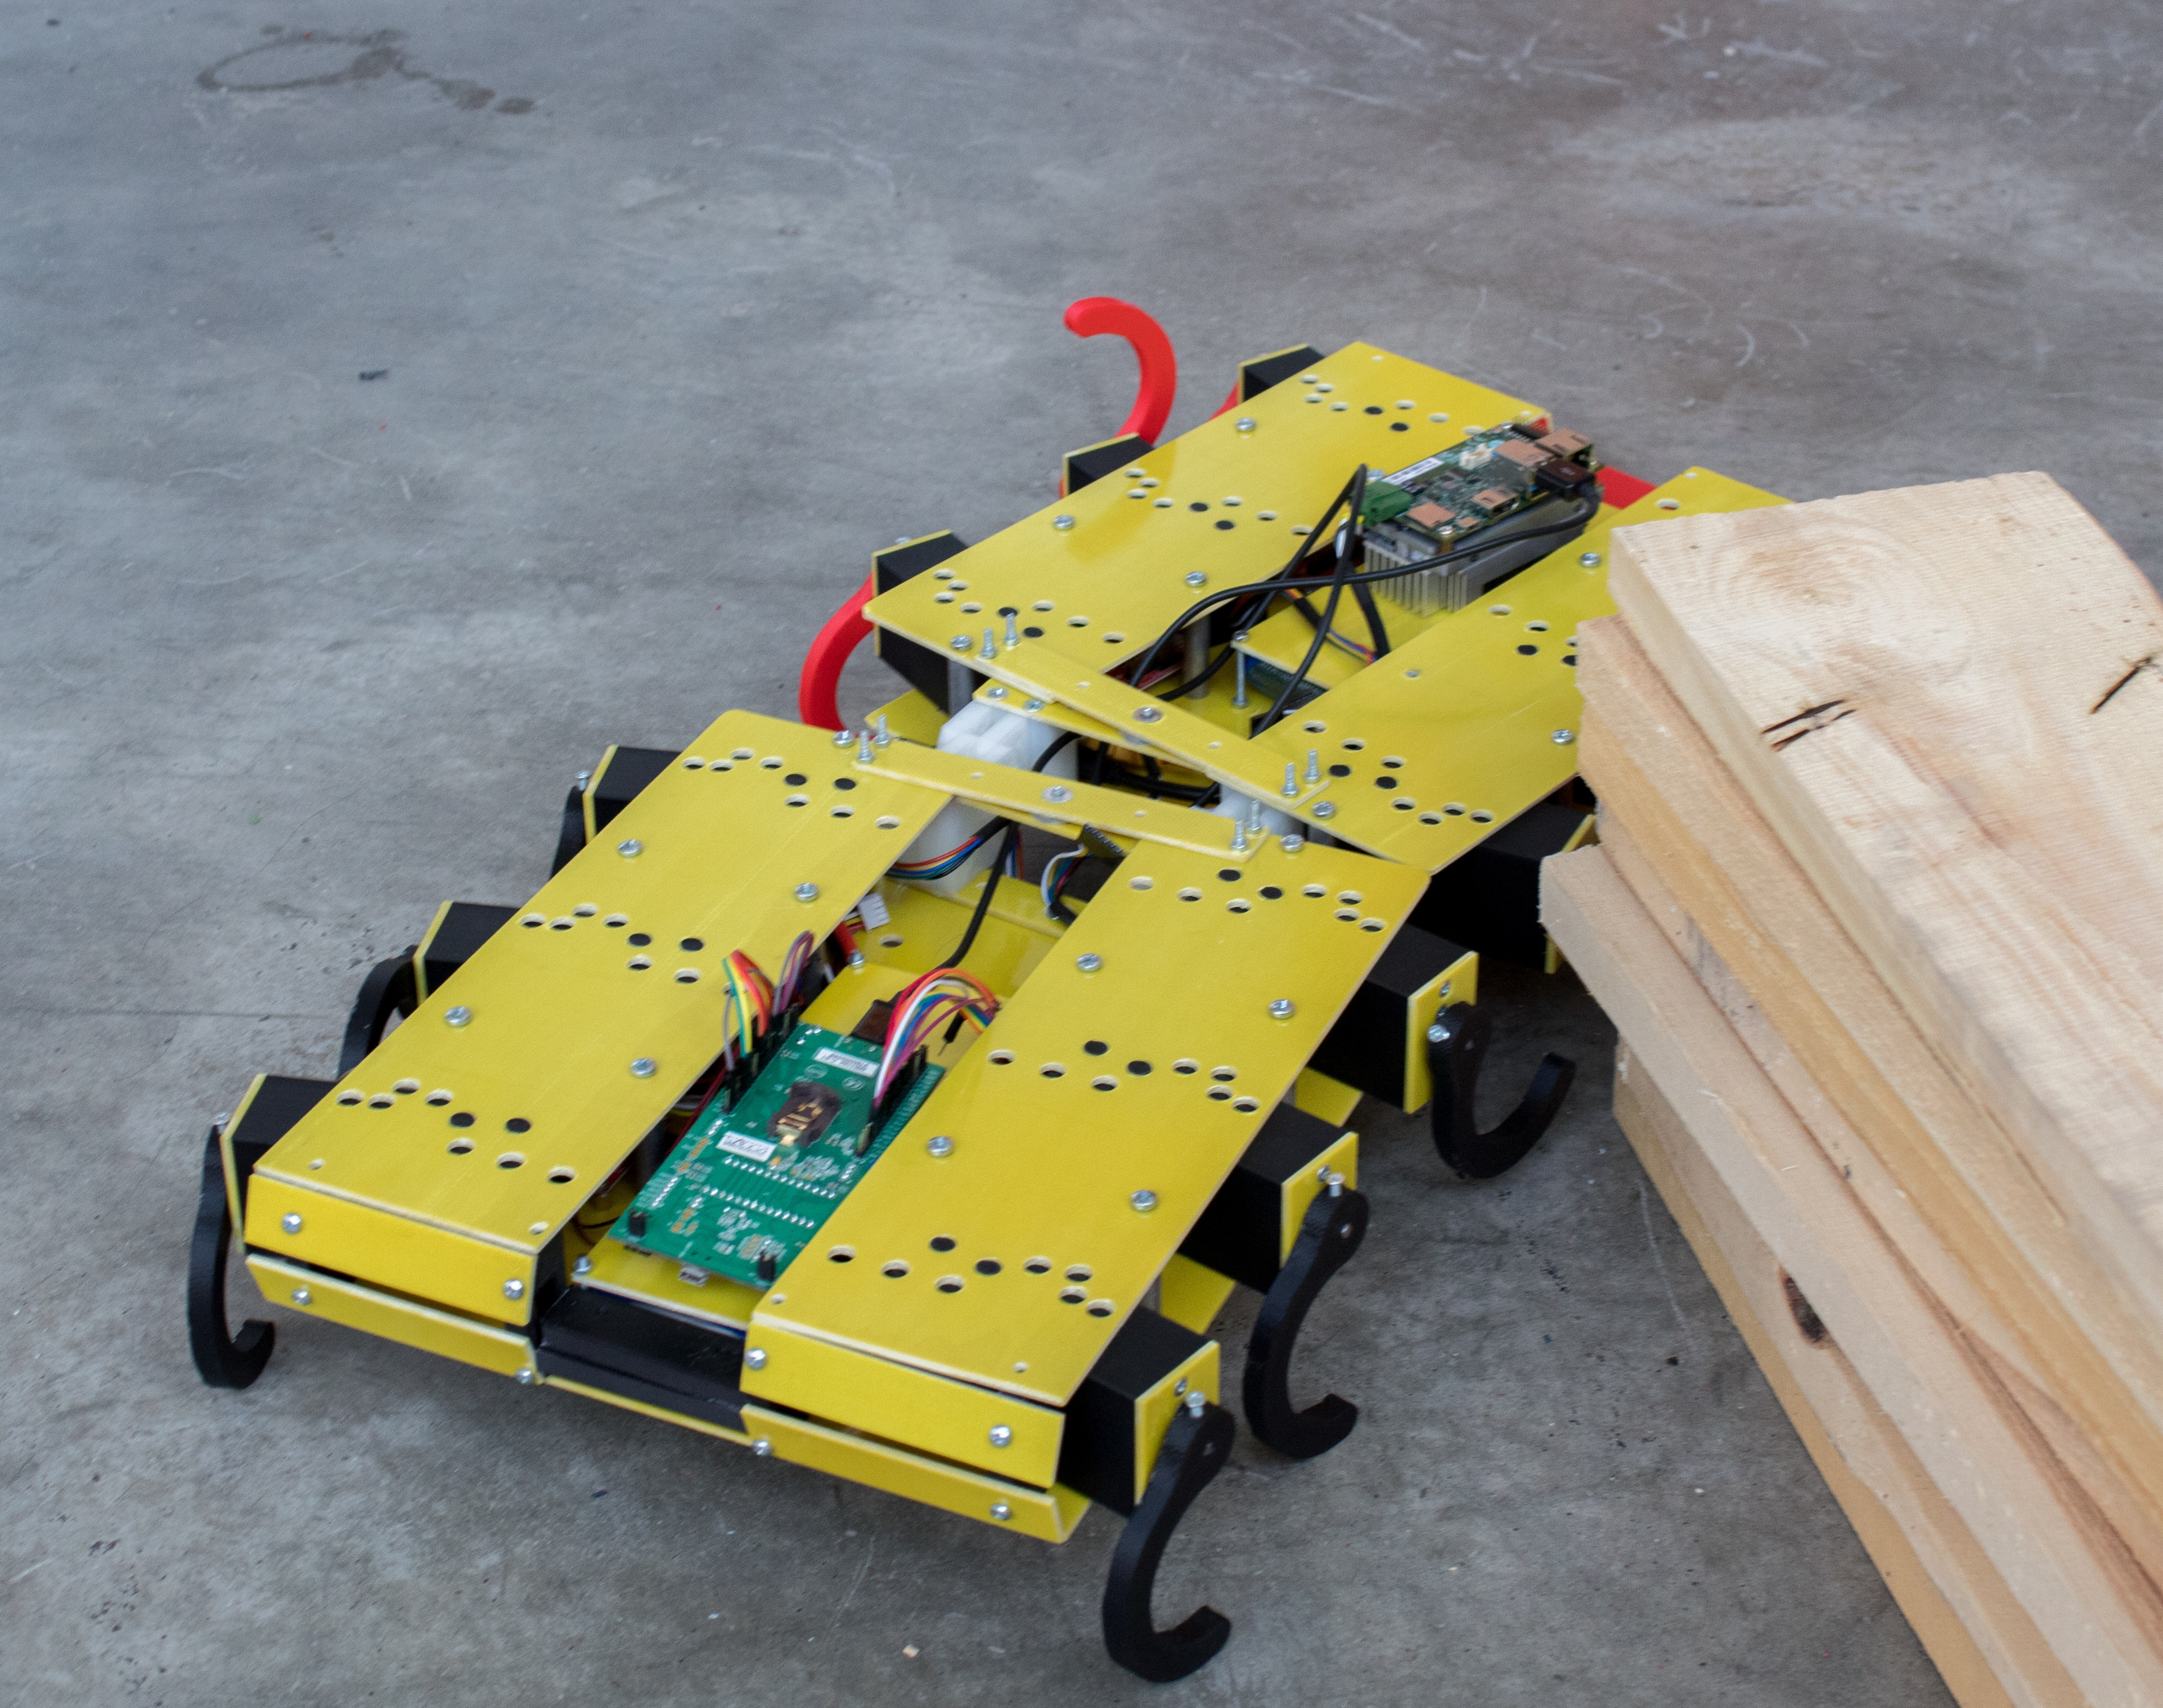
\includegraphics[width=0.33\linewidth]{strirus_2.jpg}}
        \hfill
        \subcaptionbox{Третья итерация, улучшенная\label{fig:strirus_3}}{%
        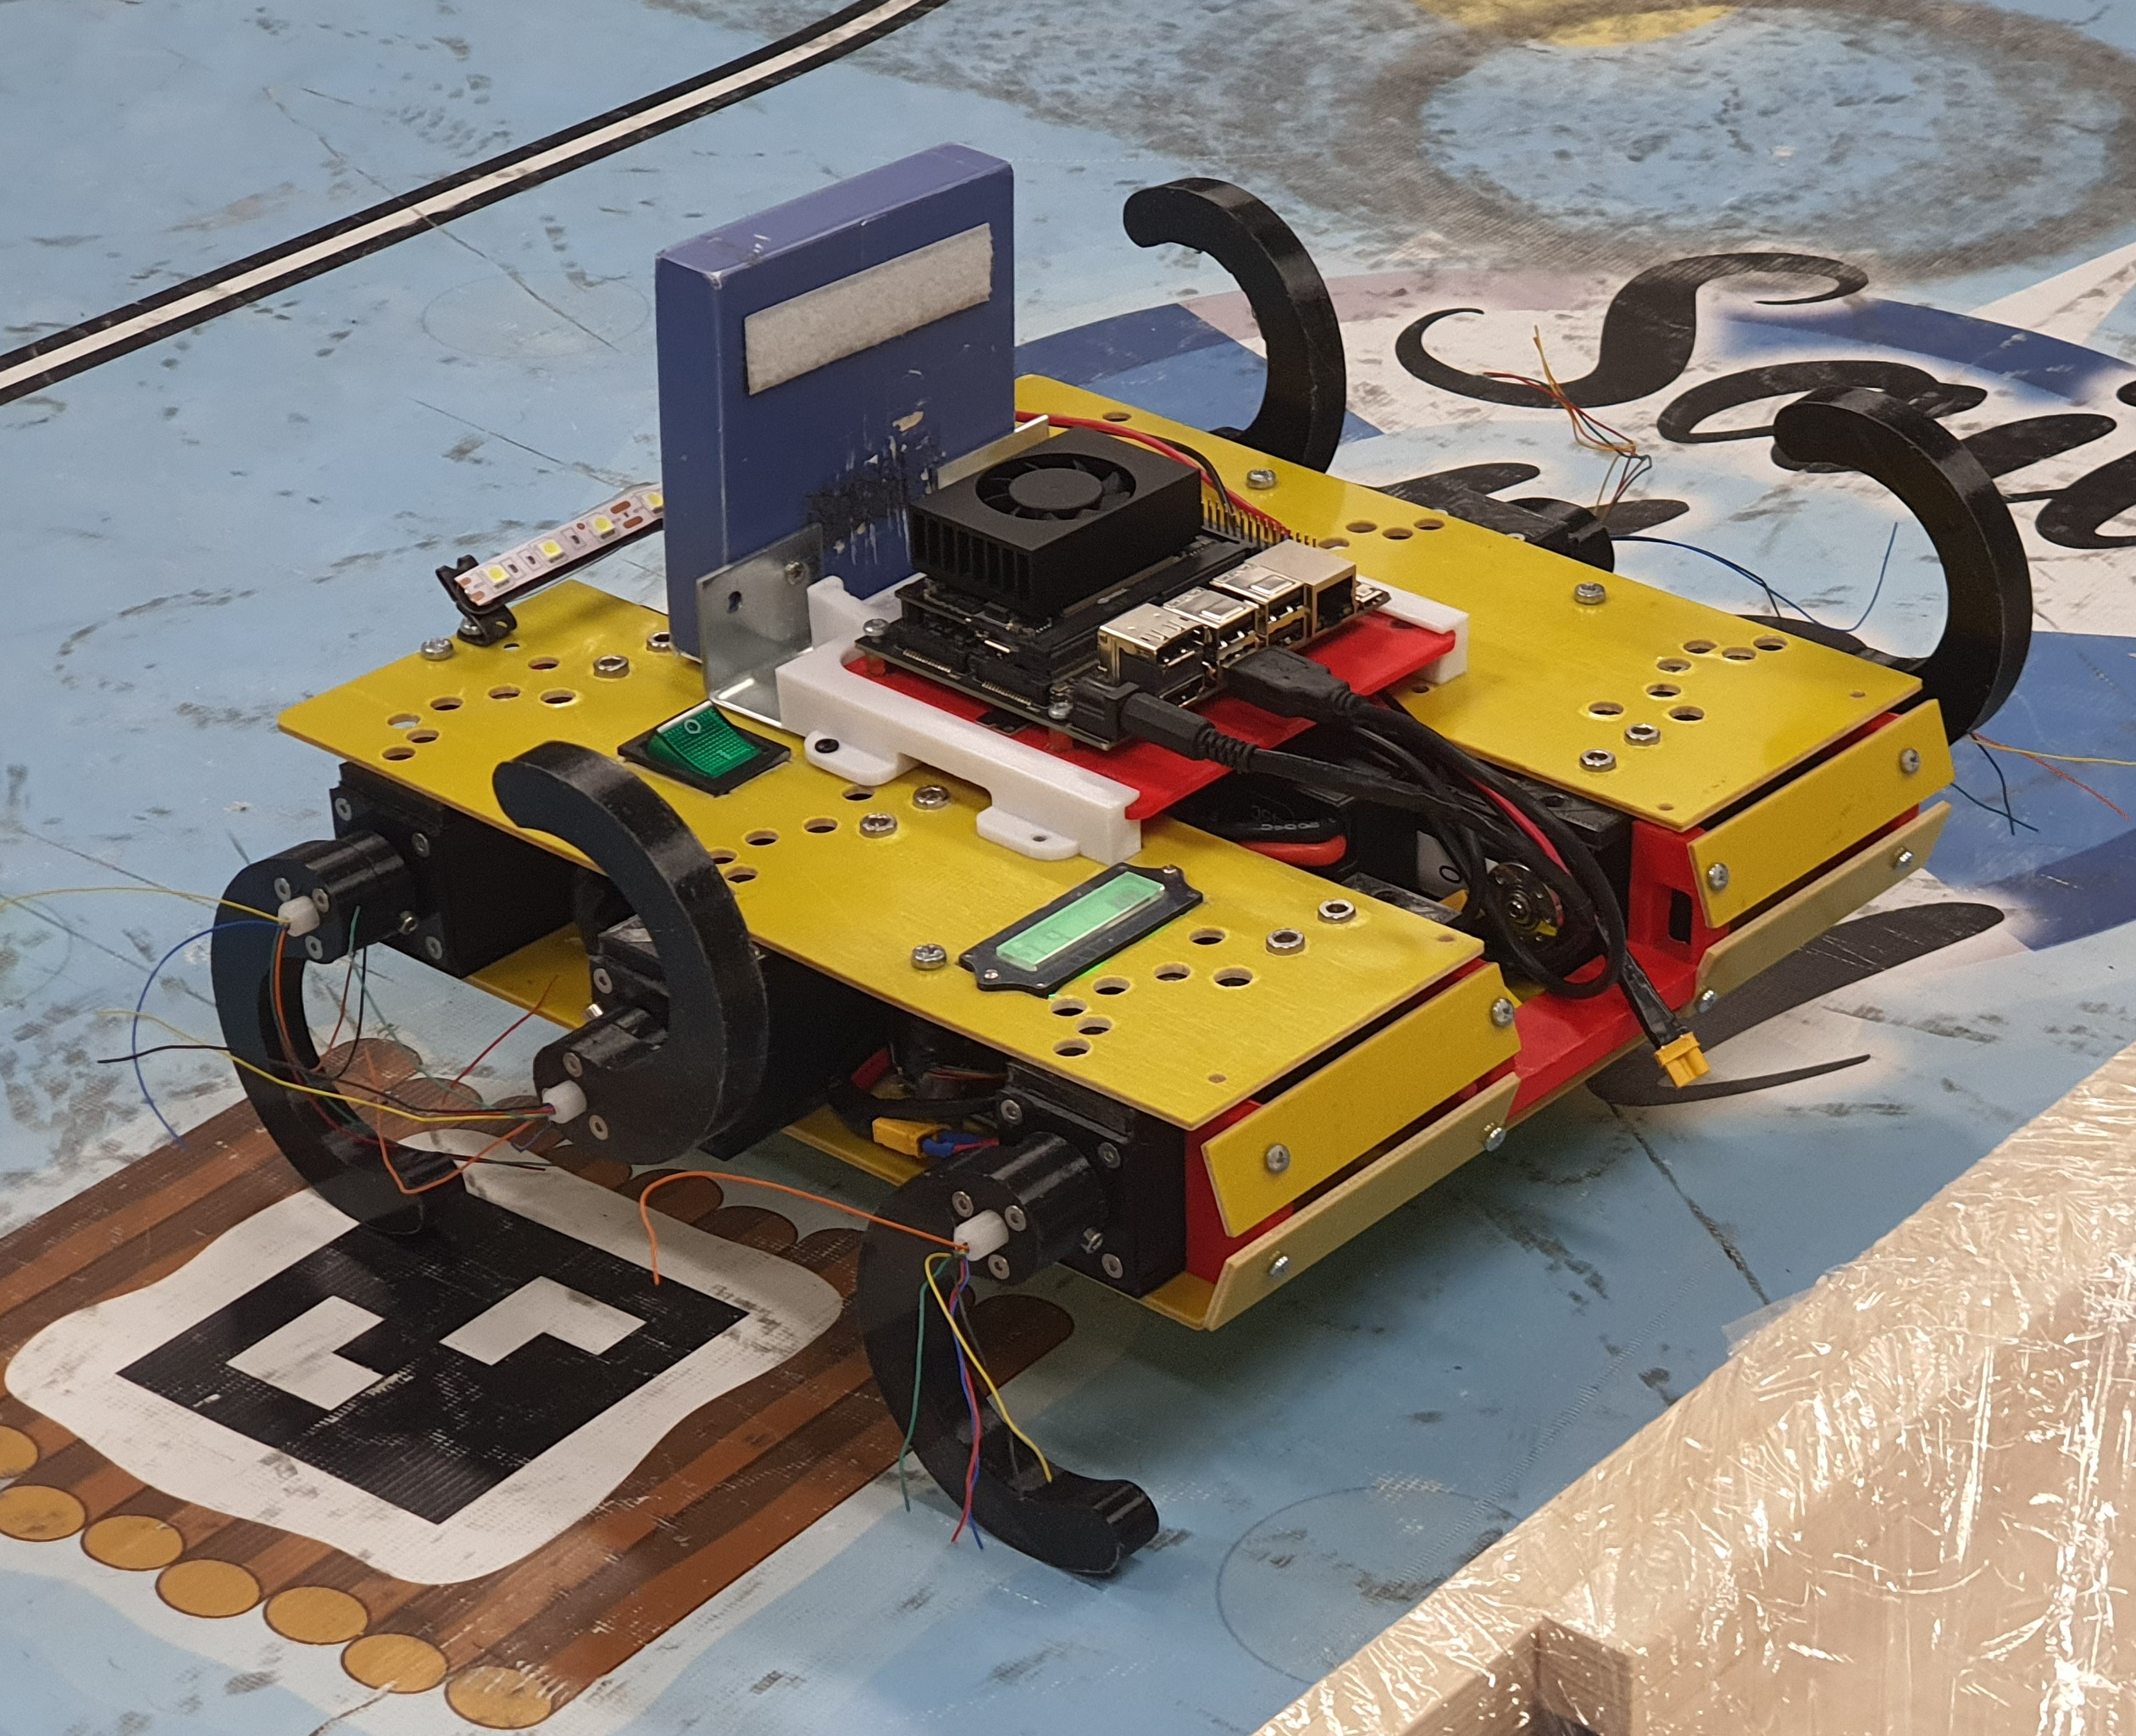
\includegraphics[width=0.45\linewidth]{strirus_3.JPG}}
        \hfill
        \subcaptionbox{Четвертая итерация\label{fig:strirus_4}}{%
        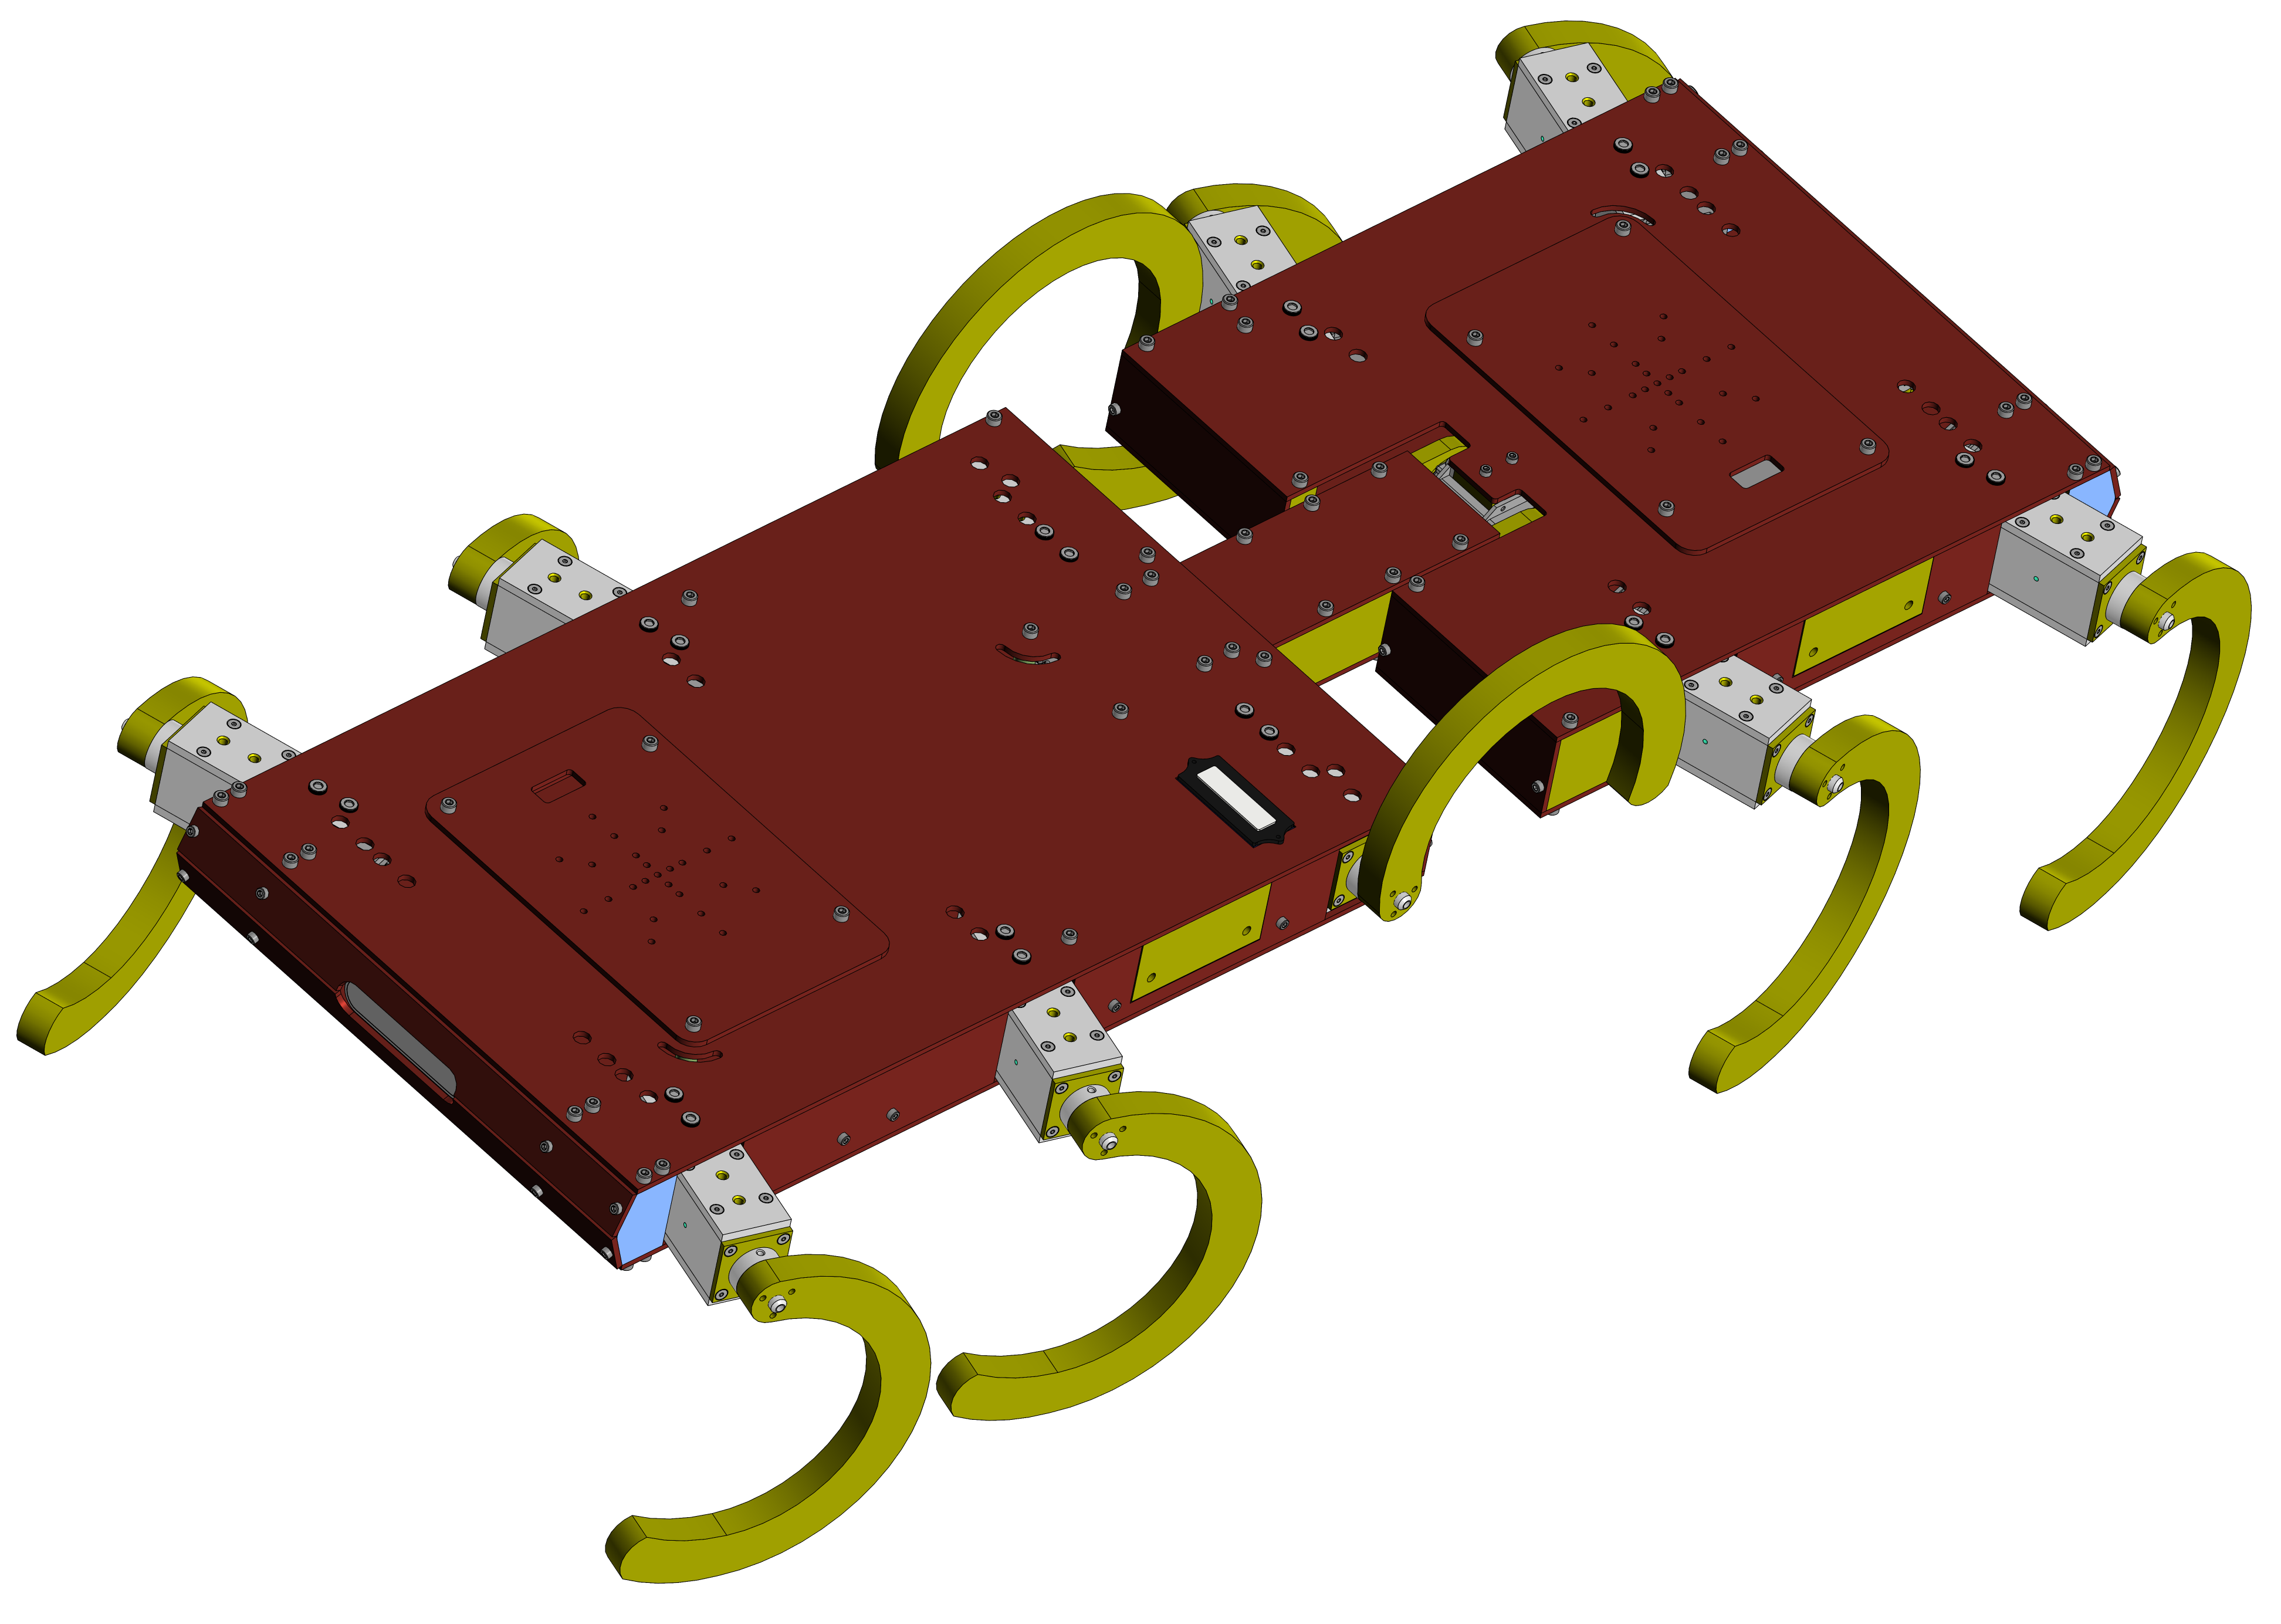
\includegraphics[width=0.45\linewidth]{strirus_4.png}}
    }
    % \legend{Подрисуночный текст, описывающий обозначения, например. Согласно
    %     ГОСТ 2.105, пункт 4.3.1, располагается перед наименованием рисунка.}
    \caption[Этот текст попадает в названия рисунков в списке рисунков]{Итерации робота СтриРуса}\label{fig:striruses}
  \end{figure}
  \vspace{-0.5cm}

\begin{table}[H]
    \caption{Сравнение итераций робота}
    \label{tabular:robot_comparison}
    % \begin{center}
    \begin{footnotesize}
    \begin{tabular}{p{1.6cm}|p{1.6cm}|p{1.5cm}|p{1.7cm}|p{1.4cm}|p{1.4cm}}
    \toprule
    \toprule
    % \rowcolor{Gray}
     Итерация & 1 \pic{fig:strirus_0}  & 2 \pic{fig:strirus_1} &  3 \pic{fig:strirus_2} & 3+ \pic{fig:strirus_3} & 4 \pic{fig:strirus_4} \\
     \hline
     Кол-во ног & 54 & 12 & 12 & 6 & 10 \\ 
    %   \rowcolor{lightgray}
     \makecell[l]{Кол-во \\ сегментов} & 1 & 2 & 2 & 1 & 2 \\
     \makecell[l]{Тип \\ соединения} & --- & Тангаж & \makecell[l]{Тангаж,\\ рыскание} & --- & Тангаж \\
    %  \rowcolor{lightgray}
     Отн. угол между телом и лапкой, градусы & 0 & 0--45 & 0, 15, 30, 45 & 0 & 0, 15 \\
     \makecell[l]{Высота \\ лапки, мм} & 54 & 60 & 60 & 90 & 170 \\
     \hline
     Особенности & Волноход & Механизм, который позволяет непрервыно изменять относительный угол & Двухстепенной узел, соединяющий сегменты & Большие лапки & Гигантские лапки  \\
    %  \rowcolor{lightgray}
    \hline
     Недостатки & Невозможно установить сенсоры на лапки. Много подвижных частей & Слишком сложный механизм, изменяющий отн. угол & Маленькие лапки. Избыточная вторая степень свободы в соединительном узле & 1 сегмент. Маленькие лапки & --- \\
    \bottomrule
    \bottomrule
    \end{tabular}
    \end{footnotesize}
    % \end{center}
    \end{table}

\subsection{Вывод}
Как итог, был разработан 10и-ногий двух сегментный робот СтриРус. 10 ног было выбрано на основе результатов, полученных во время решения мультикритериальной задачи оптимизации с помощью генетического алгоритма.

Конструкция робота соответствует всем требованиям, поставленным вначале. А именно, возможность проходить сквозь узкие пространства, иметь возможность преодолевать большие каменные гряды и возможность эффективно перемещаться по сыпучим грунтам.


